Il sensore cardiaco utilizzato è stato realizzato su una scheda PCB custom delle dimensioni di un pollice. E' composto da tre componenti: il fotodiodo VIS/IR e i due diodi LED IR e ROSSO. In Figura \ref{fig:HRS} è mostrata la disposizione dei componenti sul sensore. Si è utilizzato il datasheet dei componenti per individuare la polarità dei pin.
\begin{figure}[H]
    \centering
    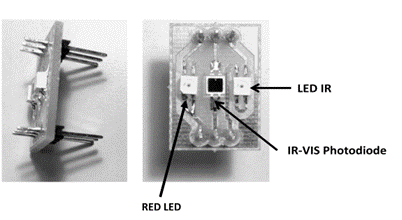
\includegraphics[width=0.5\linewidth]{Sensor.png}
    \caption{Heart Rate Sensor}
    \label{fig:HRS}
\end{figure}
Il sensore ha lo scopo di misurare la corrente erogata dal fotodiodo, il cui valore rende possibile valutare la variazione delle vene del pollice, dipendente dalla pressione sanguigna impressa dal battito del cuore.
Poiché l'uscita del fotodiodo IR/visibile è una corrente soggetta a piccole variazioni, essa risente facilmente del rumore esterno. Quindi è necessario un circuito apposito per adattare e pulire il segnale per il successivo impiego con Arduino.\\\\
Si riporta in Figura \ref{fig:Circuit} lo schematico del circuito analogico.
\begin{figure}[H]
    \centering
    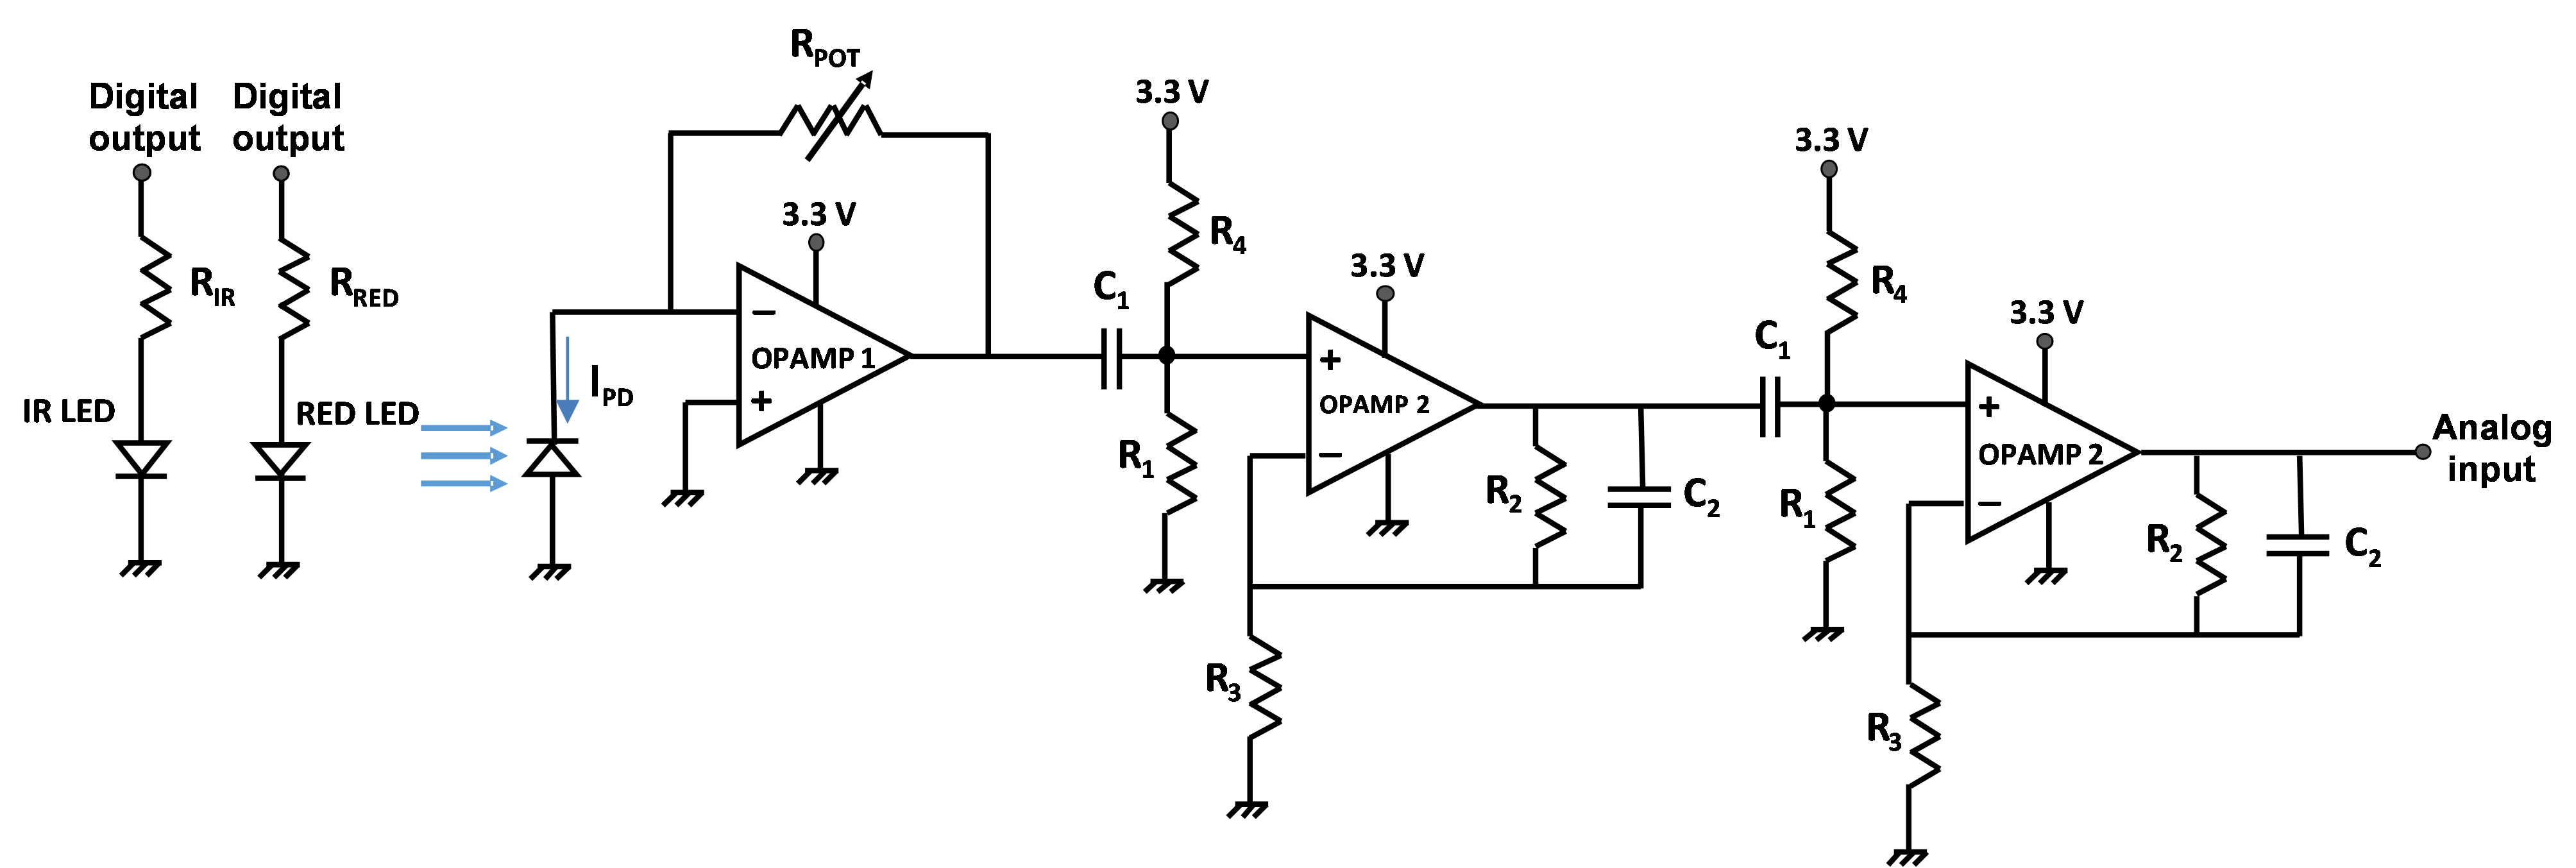
\includegraphics[width=\linewidth]{Circuit1.png}
    \caption{Schema circuito cardiofrequenzimetro/plussometro}
    \label{fig:Circuit}
\end{figure}
Il circuito è alimentato mediante porta USB del PC, la quale eroga circa $(\sim 5 V)$. Ed è composto da un primo stadio (OPAMP 1) amplificatore e un secondo stadio in cui vi è un doppio filtro passa-banda (OPAMP 2) che taglia le frequenze inferiori a 0.8 Hz e superiori a 3 Hz.\\\\
\subsection{Dimensionamento resistenze LED}
Si dimensionano le resistenze $R_{IR},R_{RED}$ in modo da ottenere sui due LED rosso e infrarosso correnti pari a $I_{RED}=15\text{ mA},I_{IR}=$3 mA rispettivamente. Usando i pin high current della scheda Arduino Due che riescono riescono ad erogare una corrente massima di 15 mA.
\begin{equation}
    \frac{V_{CC}-V_{f,IR}}{I_{IR}}=100\text{ }\Omega\quad\frac{V_{CC}-V_{f,RED}}{I_{RED}}=103.33\text{ }\Omega
\end{equation}
Dove i valori della tensione di Forward sono stati reperiti dal datasheet e valgono $V_{f,IR}=3$ V e $V_{f,RED}=1.75$ V. Quindi è stato scelto il valore commerciale più vicino per le resistenze $R_{RED} = R_{IR} = 100\text{ }\Omega$.
\subsection{Calcolo funzioni di trasferimento}
Si è anzitutto determinata la funzione di trasferimento:
\begin{itemize}
    \item Filtro passa-alto costituito da $C_1,R_1,R_4$. 
    \begin{equation}
        H_{PA}(s)=\left(1+\frac{R_2}{R_3}\right)\frac{sC_1R_1}{1+sC_1R_1}
    \end{equation}
    \item Filtro passa-basso costituito da $C_2,R_2,R_3$
    \begin{equation}
        H_{PB}(s)=-\frac{R_2}{R_3}\frac{1}{1+sC_2R_2}
    \end{equation}
    \item Filtro passa-banda complessivo
    \begin{equation*}
        H_{B}(s)=\left(1+\frac{R_2}{R_3}\right)\frac{sC_1R_1}{1+sC_1R_1}(-\frac{R_2}{R_3})\frac{1}{1+sC_2R_2}
    \end{equation*}
\end{itemize}
\subsection{Dimensionamento resistenze filtro}\label{ch:dim}
Si dimensionano le resistenze $R_1, R_2, R_3, R_4$ in modo da ottenere:
\begin{itemize}
    \item Il filtro passa-alto costituito da $C_1, R_1, R_4$ abbia frequenza di taglio pari a 0.8 Hz
    \item La tensione DC a riposo ai morsetti $V_+$ sia pari a 0.15 V
    \item Il filtro passa-basso costituito da $R_2, R_3, C_2$ abbia frequenza di taglio pari a 3 Hz
    \item Il guadagno in DC del filtro passa-basso costituito da $R_2, R_3, C_2$ sia pari a 11   
\end{itemize}
\noindent Per il filtro passa alto si vuole 
\begin{equation}
    F_H=\frac{1}{2\pi R_1C_1}=0.8\text{ Hz}\implies R_1=19894.4\text{ }\Omega
\end{equation}
\begin{equation}
    V_{Offs}=3.3\cdot\frac{R_1}{R_1+R_4}=0.15\text{ V}\implies R_4=\frac{3.3\cdot R_1}{V_{Offs}}-R_1=417782.4\text{ }\Omega
\end{equation}
Quindi è stato scelto il valore commerciale più vicino per le resistenze. Si è deciso di utilizzare $R_1 = 22k\Omega$ e $R_4 = 470k\Omega$.\\\\
Per il filtro passa basso:
\begin{equation}
    F_L=\frac{1}{2\pi R_2C_2}=3\text{ Hz}\implies R_2 = 53051.7\text{ }\Omega
\end{equation}
\begin{equation}
    A=\left|\frac{R_2}{R_3}\right|=11\implies R_3=\frac{R_2}{11}=4822.9\text{ }\Omega
\end{equation}
Quindi è stato scelto il valore commerciale più vicino per le resistenze. Si è deciso di utilizzare $R_2 = 53k\Omega$ e $R_3 = 5.6k\Omega$.
Si riassume in Tabella \ref{tab:R-value} i valori delle resistenze commerciali usate
\begin{table}[H]
    \centering
    \begin{tabular}{|c|c|}
        \hline
        $R_1$&$22\text{ k}\Omega$\\\hline
        $R_2$&$53\text{ k}\Omega$\\\hline
        $R_3$&$5.6\text{ k}\Omega$\\\hline
        $R_4$&$470\text{ k}\Omega$\\\hline
    \end{tabular}
    \caption{Valori resistenze filtri}
    \label{tab:R-value}
\end{table}
Con i valori delle resistenze scelti al punto \ref{ch:dim} e riportati in Tabella \ref{tab:R-value} otteniamo le seguenti frequenze di taglio:
\begin{equation*}
    F_L=0.723\text{ Hz}\quad F_H=3\text{ Hz}
\end{equation*}
\subsection{Tracciamento risposta in frequenza filtro}
E' stata poi tracciata la risposta in frequenza del:
\begin{itemize}
    \item Filtro passa-alto costituito da $C_1,R_1,R_4$
    \item Filtro passa-basso costituito da $C_2,R_2,R_3$
    \item Filtro passa-banda complessiva.
\end{itemize}
Nella Figura \ref{fig:bode} sono riportati i diagrammi di bode dei filtri, ottenuti con SPICE.
\begin{figure}[H]
    \centering
    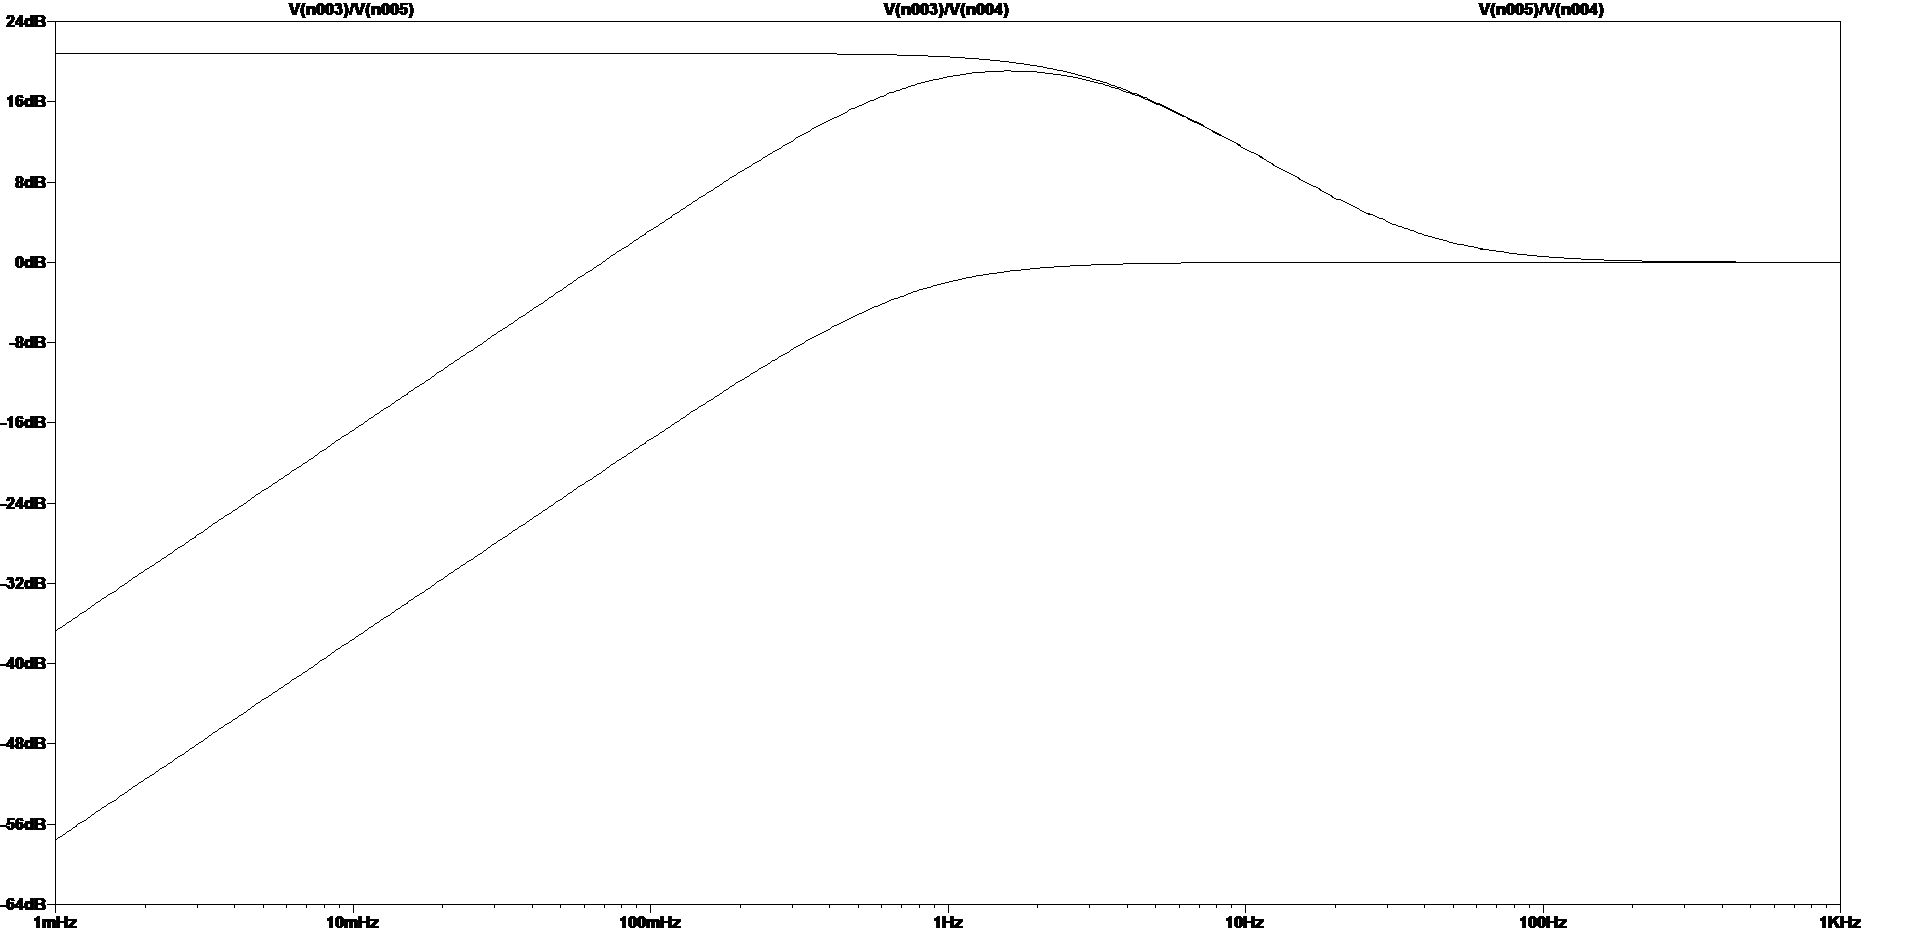
\includegraphics[width=\linewidth]{bode.png}
    \caption{Diagrammi di Bode del filtro}
    \label{fig:bode}
\end{figure}
Il grafico più altro è quello del filtro passa-basso, quello in basso è il passa-alto mentre quello complessivo passa-banda è in mezzo, come combinazione dei due filtri.